\documentclass[12pt]{article}

\usepackage{sbc-template}
\usepackage{graphicx,url}
\usepackage[utf8]{inputenc}
\usepackage[brazil]{babel}
\usepackage{amsmath}
\usepackage{tabularx}
\usepackage{array}
\usepackage{float}

\sloppy

\title{Modelagem Preditiva de Manchas Criminais: Análise Espaço-Temporal de Roubos e Furtos na Região Metropolitana de São Paulo}

\author{Aaron F. do A. M. da Silva\inst{1}, Marcos M. da Silva Filho\inst{2}, Pedro H. S. Matos\inst{3}}

\address{Escola de Artes, Ciências e Humanidades -- Universidade de São Paulo (USP)
  \email{aaronferrazamaral@usp.br, marcos\_filho@usp.br, pedrom07@usp.br}
}

\raggedbottom
\begin{document}

\maketitle

\begin{resumo}
O enfrentamento da criminalidade urbana exige abordagens analíticas capazes de apoiar o planejamento estratégico em segurança pública. Este projeto investiga o desenvolvimento de um modelo preditivo baseado em aprendizado de máquina para identificar e mapear áreas de maior risco de ocorrências patrimoniais na Região Metropolitana de São Paulo. Para isso, são utilizados dados da Secretaria de Segurança Pública do Estado de São Paulo referentes ao período de 2022 ao primeiro semestre de 2026. Inicialmente, o estudo foi direcionado aos roubos; entretanto, a Análise Exploratória dos Dados revelou limitações relacionadas ao volume de registros e à identificação de tipologias específicas, motivando a avaliação da inclusão de furtos no escopo da modelagem. Serão comparados os algoritmos Random Forest, XGBoost e LightGBM, com avaliação por métricas de regressão e por uma métrica espacial de identificação de \textit{hotspots}. Os resultados preditivos deverão ser representados por meio de mapas de risco, permitindo analisar padrões espaço-temporais das ocorrências na região estudada.
\end{resumo}

\vspace{0.5cm}

\section{Introdução}

A criminalidade urbana, especialmente os crimes contra o patrimônio, constitui um desafio relevante para o planejamento da segurança pública em regiões densamente povoadas. Na Região Metropolitana de São Paulo (RMSP), a distribuição das ocorrências não é uniforme entre os municípios nem ao longo do tempo, o que torna necessária a análise conjunta das dimensões espacial e temporal para identificar áreas de maior concentração de delitos. Nesse contexto, técnicas de Ciência de Dados e aprendizado de máquina (\textit{Machine Learning}) podem ser utilizadas para explorar padrões presentes em grandes bases de ocorrências e apoiar a construção de modelos capazes de estimar o risco associado a diferentes unidades espaço-temporais.

Este trabalho foi inicialmente concebido com foco na predição de roubos. Entretanto, durante o pré-processamento e a Análise Exploratória dos Dados (AED), foram identificadas limitações importantes para essa definição inicial. O volume de registros exclusivamente relacionados a roubos mostrou-se menor do que o esperado e, além disso, a base apresenta dificuldade para distinguir determinadas tipologias específicas de roubo. Em contrapartida, a inclusão dos registros de furto amplia consideravelmente o conjunto de dados disponível. Por essa razão, o escopo definitivo da modelagem ainda será avaliado, considerando a possibilidade de prever roubos e furtos de forma mais geral ou restringir a análise a categorias específicas relacionadas a pedestres.

A distinção entre roubo e furto também é relevante para a interpretação do problema. Embora ambos correspondam à subtração de bens, o roubo envolve violência ou grave ameaça contra a vítima, enquanto o furto ocorre sem esses elementos. Dessa forma, apesar de poderem ser analisados conjuntamente como crimes patrimoniais, as duas categorias não devem ser consideradas necessariamente homogêneas, pois representam ocorrências de naturezas distintas.

Além da definição do escopo criminal, a AED revelou dois desafios centrais para a modelagem. O primeiro é a forte concentração das ocorrências no município de São Paulo, responsável por mais de 70\% dos registros da base analisada, o que pode fazer com que os padrões da capital exerçam maior influência sobre o aprendizado do modelo. O segundo é a elevada granularidade espacial da base agregada quando são utilizadas latitude e longitude exatas. Nessa configuração, a maior parte das unidades espaço-temporais contém apenas uma ocorrência, reduzindo a repetição necessária para a aprendizagem de padrões locais. A agregação das coordenadas em um \textit{grid} espacial mostrou-se uma alternativa mais adequada e será aprofundada nas próximas etapas.

Diante desses aspectos, o objetivo deste trabalho é investigar uma estratégia de modelagem preditiva espaço-temporal capaz de estimar a quantidade de ocorrências em diferentes regiões da RMSP e, posteriormente, representar essas estimativas por meio de mapas preditivos de risco. Para isso, serão comparados os algoritmos Random Forest, XGBoost e LightGBM, considerando tanto a qualidade das previsões numéricas quanto a capacidade de identificar espacialmente áreas com maior concentração de ocorrências futuras.

\begin{figure}[ht]
\centering
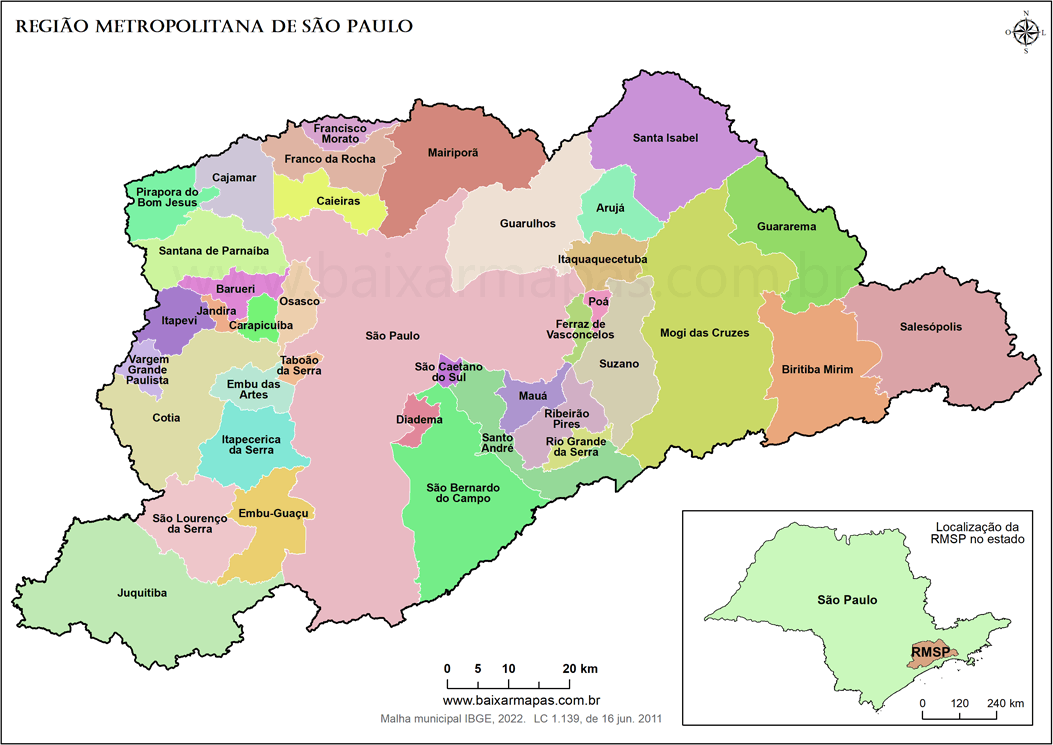
\includegraphics[width=.7\textwidth]{mapa-regiao-metropolitana-sao-paulo-municipios.png}
\caption{Região Metropolitana de São Paulo \cite{baixarmapas2026}}
\label{fig:mapa_rmsp}
\end{figure}

\vspace{1.2cm}

\section{Trabalhos Relacionados}

A aplicação de técnicas de ciência de dados e aprendizado de máquina à segurança pública tem ampliado as possibilidades de compreender padrões criminais, estimar riscos e subsidiar ações de prevenção. No contexto brasileiro, estudos recentes têm explorado diferentes recortes geográficos, categorias criminais e algoritmos preditivos. Esta seção apresenta trabalhos relacionados à identificação de padrões de crimes, à previsão de roubos e à análise dos fatores associados à criminalidade, destacando suas contribuições e a distinção da proposta desenvolvida neste trabalho.

Couto \cite{couto2024identificaccao} investigou padrões comportamentais e espaciais relacionados ao roubo de celulares no estado do Rio Grande do Sul, com ênfase no município de Porto Alegre. O autor empregou uma abordagem orientada a dados, utilizando o algoritmo não supervisionado K-means em conjunto com variáveis geográficas e sociodemográficas. A análise permitiu identificar agrupamentos territoriais associados à maior incidência desse tipo de ocorrência, evidenciando a concentração tanto de vítimas quanto de autores em bairros periféricos caracterizados por menor renda e menores indicadores de desenvolvimento humano. O estudo demonstra a relevância da integração entre dados criminais, informações territoriais e indicadores sociais para a compreensão da dinâmica espacial da criminalidade.

No trabalho de Coelho et al. \cite{de2025previsao}, foram comparados modelos de Árvores de Decisão e Redes Neurais para a previsão de roubos de veículos no município do Rio de Janeiro. Os autores avaliaram o potencial dos algoritmos de aprendizado de máquina para antecipar ocorrências e apoiar o planejamento de ações de segurança. Embora as Redes Neurais tenham apresentado melhor desempenho preditivo no estudo, os autores salientam que modelos mais complexos podem apresentar menor interpretabilidade. Essa limitação é especialmente relevante em aplicações de segurança pública, nas quais a compreensão dos fatores associados às previsões pode ser tão importante quanto a precisão do modelo para fundamentar decisões operacionais e estratégicas.

Por sua vez, Fernandes \cite{fernandes2025aplicaccao} analisou fatores socioeconômicos e estruturais associados às ocorrências criminais nos municípios do estado de São Paulo, considerando dados do período de 2008 a 2012. O estudo utilizou o algoritmo XGBoost para modelar a relação entre variáveis explicativas e a criminalidade, reportando coeficiente de determinação de 98,5%. Além do desempenho do modelo, destaca-se o uso dos valores SHAP (\textit{SHapley Additive exPlanations}) para interpretar a influência das variáveis no resultado estimado. Dessa forma, o trabalho reforça a importância de combinar modelos preditivos de alto desempenho com técnicas de interpretabilidade, permitindo analisar não apenas a previsão produzida, mas também os fatores que a explicam.

Apesar das contribuições apresentadas, os estudos identificados possuem escopos distintos quanto ao tipo de crime, à área de estudo, ao período analisado e à finalidade da modelagem. Couto \cite{couto2024identificaccao} concentra-se na identificação de agrupamentos espaciais para roubos de celulares; Coelho et al. \cite{de2025previsao} priorizam a comparação de algoritmos para roubos de veículos; e Fernandes \cite{fernandes2025aplicaccao} investiga fatores associados à criminalidade em nível municipal. Em comum, os trabalhos evidenciam o potencial de métodos orientados a dados para apoiar o diagnóstico e a prevenção da violência, mas não abordam simultaneamente a modelagem comparativa de diferentes algoritmos, a dimensão espaço-temporal e a representação cartográfica de áreas de risco na Região Metropolitana de São Paulo (RMSP).

Assim, o presente trabalho propõe uma análise aplicada à RMSP, considerando o período entre 2022 e o primeiro semestre de 2026. A pesquisa buscará examinar diferentes categorias de roubos e furtos, cuja definição final será orientada pelos resultados da análise exploratória dos dados. A etapa de modelagem comparará os algoritmos Random Forest, XGBoost e LightGBM, visando identificar abordagens adequadas à predição de ocorrências a partir de dados tabulares. Adicionalmente, pretende-se incorporar a dimensão espacial dos registros por meio da representação cartográfica das áreas de maior risco. Dessa maneira, a proposta busca contribuir para uma compreensão integrada da distribuição territorial e do comportamento temporal das ocorrências, oferecendo subsídios para o planejamento de políticas e estratégias de segurança pública.

Uma diferença metodológica relevante entre os trabalhos está na natureza da tarefa de aprendizado. Couto \cite{couto2024identificaccao} utiliza agrupamento não supervisionado para descrever concentrações e perfis territoriais já observados. Essa abordagem é apropriada para a identificação exploratória de padrões, mas não tem como objetivo estimar explicitamente o risco em períodos futuros. Por outro lado, Coelho et al. \cite{de2025previsao} e Fernandes \cite{fernandes2025aplicaccao} empregam técnicas supervisionadas, nas quais os modelos aprendem relações entre variáveis de entrada e uma variável-alvo. A proposta deste trabalho aproxima-se desse segundo grupo por estimar uma medida de risco, mas preserva a dimensão cartográfica enfatizada no primeiro, uma vez que os resultados são associados a células espaciais e convertidos em mapas de risco.

Essa distinção também influencia a forma de avaliação. Estudos voltados à explicação de fatores associados à criminalidade podem privilegiar métricas de ajuste global e técnicas de interpretabilidade, como os valores SHAP utilizados por Fernandes \cite{fernandes2025aplicaccao}. Em aplicações preditivas, contudo, é necessário verificar se o modelo mantém seu desempenho quando aplicado a períodos posteriores aos empregados no treinamento. Por essa razão, este trabalho adota uma divisão temporal entre treino, validação e teste, evitando a mistura aleatória de registros de períodos distintos. Tal cuidado é particularmente importante em segurança pública, pois mudanças sazonais, alterações no registro das ocorrências e transformações na dinâmica urbana podem comprometer a generalização de modelos treinados apenas com dados passados.

Outro aspecto pouco explorado de forma conjunta nos trabalhos selecionados é a comparação com linhas de base simples. Um modelo complexo só apresenta utilidade adicional quando supera estratégias de referência que já capturam a persistência espacial do fenômeno, como a média histórica de ocorrências em cada área. No presente estudo, a média histórica por célula H3 é empregada como referência explícita. Essa comparação permite distinguir ganhos efetivos de situações em que o padrão espacial persistente, por si só, explica grande parte da variação observada. Assim, a análise não se limita a selecionar o algoritmo com menor erro, mas examina se a sofisticação do modelo se traduz em melhoria mensurável frente a uma alternativa operacionalmente simples.

Por fim, a escala espacial diferencia a presente proposta. Enquanto os estudos relacionados analisam bairros, municípios ou recortes urbanos específicos, este trabalho utiliza células H3 para representar unidades territoriais regulares na RMSP. Essa escolha busca reduzir a dependência de limites administrativos e permitir uma representação mais detalhada da heterogeneidade espacial. A combinação entre células H3, agregação temporal por quinzena, validação cronológica e comparação com uma linha de base espacial constitui, portanto, o principal recorte metodológico desta pesquisa. Além da qualidade numérica das previsões, a etapa posterior deverá avaliar se as áreas classificadas como de maior risco são espacialmente úteis para apoiar a priorização de ações preventivas.

\begin{table}[!htbp]
\centering
\caption{Comparativo entre abordagens da literatura e o presente trabalho}
\label{tab:comparativo}
\small
\renewcommand{\arraystretch}{1.3}

\begin{tabular}{|p{2.5cm}|p{3.2cm}|p{4.0cm}|p{4.0cm}|}
\hline
\textbf{Referência} & \textbf{Método} & \textbf{Dados utilizados} & \textbf{Contribuição deste trabalho} \\
\hline

Couto \cite{couto2024identificaccao} &
K-means e análise espacial integrada a variáveis sociodemográficas &
Registros de roubo de celulares no Rio Grande do Sul, com destaque para Porto Alegre, além de informações geográficas e socioeconômicas &
Amplia a análise espacial para a RMSP e incorpora uma perspectiva preditiva e temporal, considerando diferentes categorias de roubos e furtos. \\
\hline

Coelho et al. \cite{de2025previsao} &
Árvores de Decisão e Redes Neurais &
Dados de roubos de veículos no município do Rio de Janeiro &
Compara Random Forest, XGBoost e LightGBM em outro contexto territorial e criminal, associando a predição à identificação cartográfica de áreas de maior risco. \\
\hline

Fernandes \cite{fernandes2025aplicaccao} &
XGBoost e interpretação por valores SHAP &
Indicadores socioeconômicos e estruturais dos municípios do estado de São Paulo, entre 2008 e 2012 &
Atualiza o recorte temporal para 2022--2026, focaliza a RMSP e privilegia a análise espaço-temporal das ocorrências criminais. \\
\hline

\textbf{Presente trabalho} &
Comparação entre Random Forest, XGBoost e LightGBM, com análise espacial e temporal &
Registros de roubos e furtos na RMSP entre 2022 e o primeiro semestre de 2026, complementados por variáveis disponíveis na base de dados &
Integra avaliação comparativa de modelos preditivos, análise de diferentes categorias criminais e representação cartográfica das áreas com maior risco de ocorrência. \\
\hline

\end{tabular}
\end{table}

\vspace{1.2cm}

\section{Metodologia}

Para o desenvolvimento do estudo, foi utilizada a base de dados criminais da Secretaria de Segurança Pública do Estado de São Paulo (SSP-SP)\footnote{\url{https://www.ssp.sp.gov.br/estatistica/consultas} Acesso em: 22/08/2026}, abrangendo o período de 2022 ao primeiro semestre de 2026. As diferentes fontes foram unificadas em um único conjunto de dados e, posteriormente, filtradas para manter os registros de roubos e furtos pertencentes aos municípios da Região Metropolitana de São Paulo. Embora o projeto tenha sido inicialmente direcionado aos roubos, a inclusão dos furtos no escopo da modelagem permanece em avaliação a partir dos resultados obtidos na AED.

Após a consolidação da base, foi realizado o pré-processamento dos dados, incluindo tratamento das informações de município, datas, registros duplicados e coordenadas geográficas. Em seguida, foi conduzida uma Análise Exploratória dos Dados com o objetivo de compreender a distribuição das ocorrências entre cidades, tipos de crime e períodos, além de identificar limitações relacionadas à granularidade espacial e temporal da base.

Para representar a dimensão temporal, as ocorrências foram agrupadas por quinzena. Na dimensão espacial, a análise preliminar mostrou que o uso de latitude e longitude exatas gera unidades excessivamente granulares, com baixa repetição de ocorrências. Por esse motivo, será investigada uma agregação espacial em \textit{grid}, de forma a produzir unidades espaço-temporais mais adequadas ao aprendizado dos modelos.

A modelagem será tratada como um problema de regressão, no qual o objetivo será estimar a quantidade de ocorrências associada a cada unidade espaço-temporal. O escopo definitivo das categorias utilizadas como alvo ainda será definido, considerando os resultados da AED e a possibilidade de modelar roubos e furtos de forma geral ou categorias mais específicas.

Serão comparados os algoritmos Random Forest, XGBoost e LightGBM. O Random Forest será utilizado como modelo de referência, enquanto XGBoost e LightGBM serão empregados como alternativas para comparação de desempenho. O ajuste de hiperparâmetros e a validação deverão preservar a ordem cronológica das observações, evitando que informações futuras sejam utilizadas no treinamento de previsões referentes a períodos anteriores.

Para as etapas de treinamento e validação, será utilizada a série temporal correspondente ao período de 2022 ao primeiro semestre de 2025. O intervalo remanescente, correspondente ao segundo semestre de 2025 e ao primeiro semestre de 2026, será reservado para o teste final. Essa separação temporal busca preservar a cronologia dos dados e avaliar a capacidade de generalização dos modelos em períodos posteriores aos utilizados no treinamento.

O desempenho dos modelos será analisado por meio das métricas MAE, RMSE e $R^2$, adequadas à avaliação das previsões de regressão. Adicionalmente, será utilizado o PAI para avaliar a qualidade espacial das áreas classificadas como \textit{hotspots}. Após a validação, as previsões deverão ser representadas em mapas preditivos de risco para a Região Metropolitana de São Paulo.

\vspace{1.2cm}

\section{Resultados Parciais}

Esta seção registra os resultados que podem ser reproduzidos a partir dos notebooks anexados. A análise utiliza ocorrências da SSP-SP previamente associadas a células H3 de resolução 7. A unidade de observação é a combinação entre célula H3 e quinzena: para cada unidade são agregadas as contagens de furtos, roubos e crimes patrimoniais totais. O notebook de XGBoost lê 1.789.422 registros brutos e produz 51.339 observações agregadas para treino e validação, correspondentes ao período de janeiro de 2022 a junho de 2025. O intervalo de julho de 2025 a junho de 2026, com 14.419 observações agregadas, é reservado como teste temporal.

Os alvos são medidas de risco normalizadas para o intervalo entre zero e um. Para cada período mensal, o procedimento aplica a transformação $\log(1+x)$ à contagem de ocorrências e normaliza o resultado pelo percentil de 99\% daquele período, limitando valores superiores a um. Foram construídos três alvos: risco de furto, risco de roubo e risco geral, este último derivado da contagem total de crimes. A transformação reduz o efeito de valores extremos e torna os alvos comparáveis na escala numérica empregada pelos modelos. Como consequência, MAE e RMSE devem ser interpretados como erros na escala de risco normalizada, e não como números absolutos de ocorrências.

\subsection{Desenho experimental e linha de base}

O experimento com XGBoost utiliza três dobras temporais, cada uma com 12 quinzenas de validação. A primeira dobra treina o modelo até 16 de dezembro de 2023 e o valida entre 1º de janeiro e 16 de junho de 2024. A segunda dobra utiliza dados de treino até 16 de junho de 2024 e valida o segundo semestre de 2024. Por fim, a terceira dobra treina até 16 de dezembro de 2024 e valida o primeiro semestre de 2025. Essa estrutura preserva a ordem cronológica, evitando que o modelo use registros futuros para prever períodos anteriores.

Foram avaliadas duas configurações de atributos. A versão \textit{com ano} utiliza latitude, longitude, mês, quinzena e ano; a versão \textit{sem ano} remove o último atributo. As coordenadas correspondem ao centro da célula H3. A Tabela~\ref{tab:config_experimento} sintetiza esse desenho. O notebook de Random Forest anexado prepara a mesma base agregada, constrói os alvos de risco e define a mesma separação temporal. Entretanto, ele não contém células executadas com métricas finais do Random Forest. Assim, para manter a rastreabilidade dos resultados, a comparação numérica apresentada nesta seção utiliza exclusivamente as saídas persistidas do notebook de XGBoost e sua linha de base.

\begin{table}[!htbp]
\centering
\caption{Configuração do experimento reprodutível a partir dos notebooks}
\label{tab:config_experimento}
\small
\renewcommand{\arraystretch}{1.2}
\resizebox{\textwidth}{!}{%
\begin{tabular}{|l|l|l|l|}
\hline
\textbf{Elemento} & \textbf{Definição} & \textbf{Período} & \textbf{Finalidade} \\
\hline
Unidade espacial & Célula H3, resolução 7 & Toda a RMSP disponível na base & Representar o risco em unidades territoriais regulares \\
\hline
Unidade temporal & Quinzena & Jan./2022 a jun./2026 & Agregar ocorrências em intervalos temporais regulares \\
\hline
Treino e validação & 51.339 observações agregadas & Jan./2022 a jun./2025 & Ajustar modelos e escolher configurações \\
\hline
Teste temporal & 14.419 observações agregadas & Jul./2025 a jun./2026 & Avaliação final futura, ainda reservada no notebook do XGBoost \\
\hline
Validação cruzada & Três dobras temporais de 12 quinzenas & Jan./2024 a jun./2025 & Medir generalização em períodos posteriores \\
\hline
Configurações & Com ano; sem ano & Atributos espaciais e temporais & Verificar a contribuição da variável ano \\
\hline
\end{tabular}%
}
\end{table}

A linha de base é a \textit{média histórica por célula}. Em cada dobra, o risco previsto para uma célula é a média do respectivo alvo observada somente nos dados de treinamento daquela dobra. Formalmente, para a célula $h$ e o alvo $y$, a previsão de referência é dada por:

\begin{equation}
\hat{y}_{h}^{\mathrm{hist}} = \frac{1}{n_h}\sum_{i \in \mathrm{treino}(h)} y_i.
\end{equation}

Essa previsão não usa os atributos dos algoritmos e, portanto, não depende de XGBoost ou Random Forest. Contudo, ela é recalculada a cada dobra porque o conjunto de treino cresce ao longo do tempo. Por isso, as métricas apresentadas correspondem à média das três dobras, e não a uma única constante global. Para uma comparação justa, todos os algoritmos devem usar o mesmo alvo, a mesma agregação e exatamente as mesmas dobras; nessas condições, a linha de base terá o mesmo resultado para todos eles.

\subsection{Validação cruzada do XGBoost}

O XGBoost foi ajustado por busca aleatória de hiperparâmetros, com 20 combinações avaliadas para cada alvo e configuração. A busca considerou número de árvores, taxa de aprendizado, profundidade máxima, tamanho mínimo de folha, subamostragem de linhas e de atributos e regularização $L_2$. Para furto e roubo, a melhor configuração encontrada foi composta por 800 árvores, taxa de aprendizado de 0.03, profundidade 8, \textit{subsample} de 0.8, \textit{colsample\_bytree} de 0.8 e regularização $L_2$ igual a 5. Para o risco geral sem ano, a busca selecionou uma configuração menos regularizada, com \textit{subsample} igual a 1.0 e regularização igual a 1.

A Tabela~\ref{tab:xgb_cv} apresenta as médias das métricas nas três dobras. Em todos os três alvos, a média histórica por célula obteve o menor RMSE. Para risco de furto, a linha de base atingiu RMSE de 0.0715, enquanto o melhor XGBoost, com ano, alcançou 0.0730. Para risco de roubo, a diferença foi menor: 0.1008 para a média histórica e 0.1017 para o XGBoost com ano. Para o risco geral, a referência apresentou RMSE de 0.0558, em comparação com 0.0567 do melhor XGBoost.

Esses resultados mostram que a persistência espacial é uma característica forte da base: conhecer a média histórica de uma célula explica uma parcela substancial do risco futuro. Isso não significa que o XGBoost seja inadequado, mas indica que, com os atributos atualmente disponíveis, ele ainda não extraiu informação suficiente para superar uma referência espacial simples. A diferença de desempenho também é pequena, sobretudo para roubo e risco geral, o que torna inadequado concluir que um modelo é superior ao outro apenas pela complexidade do algoritmo.

\begin{table}[!htbp]
\centering
\caption{Métricas médias da validação cruzada temporal do XGBoost}
\label{tab:xgb_cv}
\scriptsize
\renewcommand{\arraystretch}{1.15}
\resizebox{\textwidth}{!}{%
\begin{tabular}{|l|l|c|c|c|c|}
\hline
\textbf{Alvo} & \textbf{Modelo} & \textbf{$R^2$} & \textbf{MAE} & \textbf{RMSE} & \textbf{DP do RMSE} \\
\hline
Risco de furto & Média histórica por célula & 0.9262 & 0.0537 & 0.0715 & 0.0004 \\
Risco de furto & XGBoost com ano & 0.9229 & 0.0551 & 0.0730 & 0.0010 \\
Risco de furto & XGBoost sem ano & 0.9204 & 0.0564 & 0.0742 & 0.0007 \\
\hline
Risco de roubo & Média histórica por célula & 0.8863 & 0.0789 & 0.1008 & 0.0034 \\
Risco de roubo & XGBoost com ano & 0.8844 & 0.0798 & 0.1017 & 0.0025 \\
Risco de roubo & XGBoost sem ano & 0.8808 & 0.0812 & 0.1033 & 0.0024 \\
\hline
Risco geral & Média histórica por célula & 0.9519 & 0.0416 & 0.0558 & 0.0015 \\
Risco geral & XGBoost com ano & 0.9502 & 0.0430 & 0.0567 & 0.0018 \\
Risco geral & XGBoost sem ano & 0.9482 & 0.0439 & 0.0579 & 0.0009 \\
\hline
\end{tabular}%
}
\end{table}

A inclusão da variável ano melhora o resultado do XGBoost em todos os alvos quando comparada à versão sem ano. A redução do RMSE é de aproximadamente 1,6\% para furto, 1,5\% para roubo e 2,1\% para risco geral. O efeito é consistente, mas não suficiente para ultrapassar a média histórica. Assim, o ano parece registrar parte da variação entre períodos, porém ainda não representa adequadamente mudanças mais finas no processo gerador das ocorrências.

\subsection{Risco geral por combinação de previsões}

Também foi avaliada uma estratégia de \textit{ensemble} para estimar o risco geral a partir das previsões separadas de furto e roubo. Foram testados três procedimentos: média simples das duas previsões, seleção do maior valor previsto e regressão linear com coeficientes positivos. A regressão foi ajustada com previsões fora da amostra das três dobras. Os pesos estimados foram 0.641 para furto e 0.325 para roubo, com intercepto de 0.068, sugerindo maior contribuição da componente de furto na composição do risco geral.

Conforme a Tabela~\ref{tab:ensemble_xgb}, a regressão linear foi a melhor estratégia de combinação, alcançando RMSE de 0.0575. O método do máximo obteve desempenho intermediário, enquanto a média simples teve o maior erro. Ainda assim, o XGBoost treinado diretamente para o risco geral apresentou RMSE de 0.0567, ligeiramente menor que o \textit{ensemble} por regressão linear. Além disso, a média histórica por célula permaneceu como melhor referência no mesmo desenho de validação, com RMSE de 0.0558.

Esse resultado indica que, nesta etapa, estimar diretamente o risco geral é mais eficiente do que combinar previsões especializadas de furto e roubo. Deve-se ainda interpretar o desempenho da regressão linear com cautela: os pesos foram aprendidos e avaliados sobre previsões fora da amostra das mesmas dobras, procedimento identificado pelo próprio notebook como levemente otimista. Uma avaliação mais rigorosa exigirá uma camada adicional de validação ou o ajuste dos pesos em uma janela temporal anterior à utilizada para avaliação.

\begin{table}[!htbp]
\centering
\caption{Combinação de previsões de furto e roubo para estimar o risco geral}
\label{tab:ensemble_xgb}
\small
\renewcommand{\arraystretch}{1.15}
\begin{tabular}{|l|c|c|c|}
\hline
\textbf{Método} & \textbf{$R^2$} & \textbf{MAE} & \textbf{RMSE} \\
\hline
Média simples & 0.8990 & 0.0633 & 0.0809 \\
Máximo & 0.9270 & 0.0526 & 0.0687 \\
Regressão linear positiva & 0.9489 & 0.0443 & 0.0575 \\
\hline
XGBoost direto para risco geral (com ano) & 0.9502 & 0.0430 & 0.0567 \\
Média histórica por célula & 0.9519 & 0.0416 & 0.0558 \\
\hline
\end{tabular}
\end{table}

\subsection{Importância dos atributos e interpretação espacial}

A Figura~\ref{fig:importancia_xgb} apresenta a importância por ganho das variáveis no XGBoost treinado para o risco geral. Em ambas as configurações, longitude e latitude concentram quase toda a importância atribuída pelo modelo. Quando o ano é incluído, sua contribuição é pequena; mês e quinzena apresentam importância praticamente nula. Esse padrão é coerente com o desempenho competitivo da média histórica por célula: a posição territorial é o principal sinal utilizado pelo modelo, enquanto os atributos temporais disponíveis acrescentam pouca informação discriminante.

O resultado não deve ser interpretado como evidência de que a temporalidade é irrelevante para a criminalidade. Ele revela apenas que as variáveis temporais empregadas --- mês, quinzena e ano --- não capturaram, nos experimentos atuais, variações temporais suficientes para gerar grande ganho de predição. Informações como tendências recentes por célula, defasagens de ocorrências, sazonalidade cíclica, feriados, mobilidade, eventos locais e alterações na dinâmica urbana podem ser mais adequadas para representar essa dimensão.

\begin{figure}[!htbp]
\centering
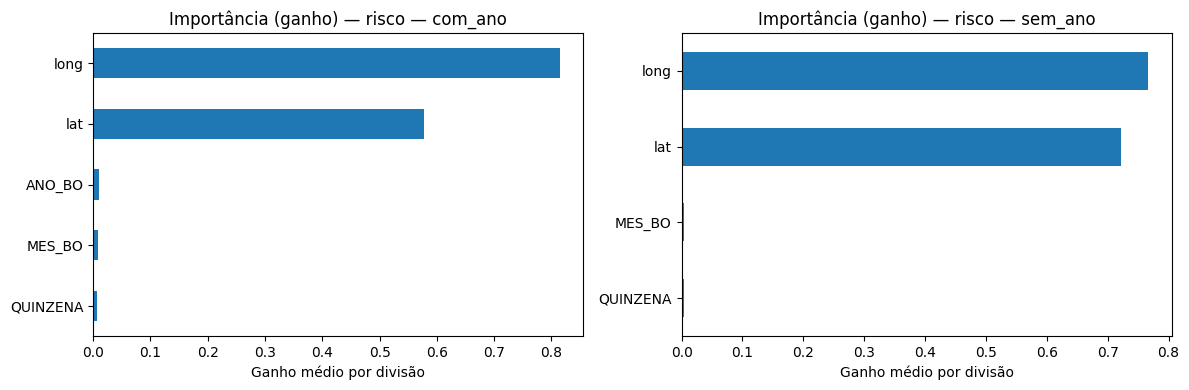
\includegraphics[width=\textwidth]{importancia_xgboost.png}
\caption{Importância por ganho das variáveis no XGBoost para risco geral. À esquerda, modelo com ano; à direita, modelo sem ano.}
\label{fig:importancia_xgb}
\end{figure}

Os resultados também reforçam a utilidade das células H3 para a representação cartográfica. Como as previsões são produzidas para unidades espaciais regulares, é possível convertê-las em mapas de risco e destacar áreas prioritárias. Contudo, a qualidade visual de um mapa não substitui a validação quantitativa. Para que a representação espacial tenha utilidade operacional, será necessário complementar MAE, RMSE e $R^2$ com métricas voltadas à priorização territorial, como a proporção de ocorrências capturada nas células classificadas entre as de maior risco, além de métricas de \textit{hotspots}, como o Predictive Accuracy Index (PAI).

\section{Discussão e Conclusão}

O estudo estruturou uma base espaço-temporal de ocorrências patrimoniais na RMSP, agregada em células H3 e quinzenas, e avaliou uma linha de base histórica e modelos de aprendizado de máquina. No experimento reprodutível de XGBoost, a média histórica por célula apresentou o menor erro para furto, roubo e risco geral. O XGBoost com ano superou consistentemente sua versão sem ano, mas não ultrapassou a referência histórica. A análise de importância das variáveis indica que latitude e longitude concentram a maior parte do ganho, o que evidencia a forte persistência espacial dos padrões observados.

O fato de a média histórica competir ou superar os algoritmos não representa uma falha isolada do modelo; trata-se de um resultado substantivo. Ele mostra que, com os atributos atuais, a localização média de risco contém mais informação preditiva do que a parcela adicional capturada pelo XGBoost. Esse diagnóstico exige cuidado metodológico: a média histórica deve ser calculada apenas com os dados de treino de cada dobra e avaliada nas mesmas células, períodos e escalas dos demais modelos. Caso agregação temporal, definição do alvo, dobras ou normalização sejam diferentes, suas métricas deixam de ser diretamente comparáveis.

Como próximo passo, recomenda-se padronizar um único protocolo de avaliação para Random Forest, XGBoost e LightGBM: mesmos alvos, mesma agregação H3--quinzena, mesmas dobras temporais, mesma linha de base e um teste final intocado entre julho de 2025 e junho de 2026. A normalização do risco também deve ser revisada para que parâmetros calculados a partir da distribuição do período de teste não incorporem informação indisponível no instante da previsão. Em seguida, podem ser incorporadas variáveis defasadas de ocorrência, sazonalidade cíclica, feriados, mobilidade, dados socioeconômicos e características urbanas.

Por fim, uma aplicação real exigirá mais do que menor RMSE. Será necessário medir a capacidade de priorizar corretamente células de alto risco, calibrar as previsões, acompanhar degradação do modelo ao longo do tempo e auditar possíveis vieses territoriais. Nessa perspectiva, o modelo deve ser empregado como apoio analítico e cartográfico para a tomada de decisão humana, com atualização periódica e avaliação contínua de seus efeitos.


\bibliographystyle{plain}
\bibliography{referencias}

\end{document}





Quantidade máxima de páginas por seção:
Título e resumo 1 página
Introdução  2 páginas
Método 2 páginas
Trabalhos correlatos 3 páginas
Resultados preliminares (análise exploratória dos dados) 3 páginas
Discussão e conclusão 1 página



Tabela 1: Comparativo entre abordagens da literatura e esse trabalho
- Colunas: Referência; Método; Dados utilizados; Contribuição deste trabalho

